\documentclass[12pt, a4paper]{article}

% ---- Packages ----
\usepackage[utf8]{inputenc}
\usepackage[T1]{fontenc}
\usepackage{amsmath, amssymb, amsfonts}
\usepackage{graphicx}
\usepackage{booktabs}
\usepackage{geometry}
\usepackage{enumitem}
\usepackage{listings}
\usepackage{xcolor}
\usepackage{titlesec}
\usepackage{caption}
\usepackage{subcaption}
\usepackage{float}
\usepackage{setspace}

\geometry{margin=1in}
\onehalfspacing

% ---- Hyperref (no colored boxes) ----
\usepackage[hidelinks]{hyperref}

% ---- Code listing style ----
\lstset{
    basicstyle=\ttfamily\small,
    breaklines=true,
    frame=single,
    backgroundcolor=\color{gray!10},
    keywordstyle=\color{blue},
    commentstyle=\color{green!50!black},
    stringstyle=\color{red}
}

% ---- Section formatting ----
\titleformat{\section}{\normalfont\Large\bfseries}{\thesection}{1em}{}
\titleformat{\subsection}{\normalfont\large\bfseries}{\thesubsection}{1em}{}

% ---- Title Page ----
\begin{document}

\begin{titlepage}
    \centering
    \vspace*{0.5cm}

    
\includegraphics[width=0.35\textwidth]{COEP_Tech_logo.jpeg}\\[0.8cm]

    {\LARGE \textbf{COEP Technological University}}\\[0.6cm]
    {\Huge \textbf{VQA Modal Analysis}}\\[0.3cm]
    {\Large Quantum Computing for Structural Dynamics}\\[1.5cm]

    {\large
    \begin{tabular}{c}
    Project Report \\[0.3cm]
    Department of Computer Science \& Engineering \\[0.8cm]
    Date: May 2026
    \end{tabular}
    }

    \vfill
\end{titlepage}

% ---- Table of Contents ----
\tableofcontents
\newpage

% ===================================================================
\section{Introduction}
% ===================================================================

Modal analysis determines the natural frequencies and mode shapes of vibrating structures. These intrinsic properties define how a structure responds to dynamic loads and are essential for resonance avoidance, fatigue prediction, and structural health monitoring.

This project demonstrates the application of the \textbf{Variational Quantum Eigensolver (VQE)} algorithm to solve structural modal analysis problems for both beam and 2D truss structures. The fundamental insight is that the generalized eigenvalue problem in structural dynamics can be transformed into a quantum eigenvalue problem:

\begin{equation}
    K\phi = \omega^2 M\phi \quad \xrightarrow{\ H = M^{-1/2} K M^{-1/2}\ } \quad H|\psi\rangle = \lambda|\psi\rangle
\end{equation}

where $\lambda = \omega^2$. This mapping enables the use of quantum algorithms to find structural natural frequencies.

% ===================================================================
\section{Theoretical Foundation}
% ===================================================================

\subsection{Structural Dynamics Eigenvalue Problem}

The equation of motion for a discretized structure is:

\begin{equation}
    M\ddot{u} + K u = 0
\end{equation}

Assuming harmonic motion $u = \phi e^{i\omega t}$, we obtain the generalized eigenvalue problem:

\begin{equation}
    K\phi = \omega^2 M\phi
\end{equation}

where:
\begin{itemize}[noitemsep]
    \item $K$ = Global stiffness matrix (N/m)
    \item $M$ = Global mass matrix (kg)
    \item $\phi$ = Mode shape eigenvector
    \item $\omega$ = Natural frequency (rad/s)
\end{itemize}

\subsection{Transformation to Quantum Eigenvalue Problem}

Since $M$ is symmetric positive definite, we compute $M^{-1/2}$ via eigendecomposition and define:

\begin{equation}
    H = M^{-1/2} K M^{-1/2}, \quad |\psi\rangle = M^{1/2}\phi
\end{equation}

The transformed problem $H|\psi\rangle = \lambda|\psi\rangle$ has eigenvalues $\lambda = \omega^2$, making it directly solvable via quantum algorithms.

\subsection{Pauli Decomposition}

For quantum computation, the Hamiltonian must be expressed as a sum of Pauli operators:

\begin{equation}
    H = \sum_i c_i P_i, \quad P_i \in \{I, X, Y, Z\}^{\otimes n}
\end{equation}

\subsection{Hamiltonian Normalization}

Structural matrices often have eigenvalues spanning multiple orders of magnitude. Normalization ensures stable VQE convergence:

\begin{equation}
    H_{\text{norm}} = \frac{H}{\|H\|}, \quad \omega = \sqrt{\lambda_{\text{vqe}} \cdot H_{\text{scale}}}
\end{equation}

% ===================================================================
\section{System Architecture}
% ===================================================================

\subsection{Pipeline Overview}

\begin{verbatim}
INPUT: Material (E, rho), Geometry (L, I/A), Mesh (n_elem)
  |
  v
FINITE ELEMENT ANALYSIS (fea.py / truss.py)
  |  Output: K_global, M_global
  v
BOUNDARY CONDITIONS
  |  Output: K_red, M_red, free_dofs
  v
QUANTUM HAMILTONIAN (quantum_setup.py)
  |  M^{-1/2} K M^{-1/2} -> Pauli decomposition
  v
VQE OPTIMIZATION (vqe_runner.py + ansatz.py)
  |  Multi-start, two-stage refinement
  v
RESULTS: Natural frequencies, mode shapes, convergence
\end{verbatim}

\subsection{Project Structure}



% ===================================================================
\section{Finite Element Analysis Modules}
% ===================================================================

\subsection{Beam Element (fea.py)}

Euler-Bernoulli beam elements with 2 DOFs per node (transverse displacement $v$ and rotation $\theta$):

\begin{equation}
k_e = \frac{EI}{L^3}
\begin{bmatrix}
12 & 6L & -12 & 6L \\
6L & 4L^2 & -6L & 2L^2 \\
-12 & -6L & 12 & -6L \\
6L & 2L^2 & -6L & 4L^2
\end{bmatrix}
\end{equation}

Consistent mass matrix:

\begin{equation}
m_e = \frac{\rho A L}{420}
\begin{bmatrix}
156 & 22L & 54 & -13L \\
22L & 4L^2 & 13L & -3L^2 \\
54 & 13L & 156 & -22L \\
-13L & -3L^2 & -22L & 4L^2
\end{bmatrix}
\end{equation}

\textbf{Boundary Conditions:} Simply-supported (pin-pin) removes transverse DOF at both ends, yielding $2n$ free DOFs for $n$ elements.

\textbf{Analytical Solution:} For a simply-supported beam:
\begin{equation}
    \omega_n = \left(\frac{n\pi}{L}\right)^2 \sqrt{\frac{EI}{\rho A}}
\end{equation}

\subsection{1D Truss Element (truss.py)}

Axial-only bar elements with 1 DOF per node:

\begin{equation}
k_e = \frac{EA}{L}
\begin{bmatrix}
1 & -1 \\ -1 & 1
\end{bmatrix}, \quad
m_e = \frac{\rho A L}{6}
\begin{bmatrix}
2 & 1 \\ 1 & 2
\end{bmatrix}
\end{equation}

\textbf{BCs:} Fixed-fixed removes DOFs at both end nodes. Analytical frequency: $\omega_n = \frac{n\pi}{L}\sqrt{\frac{E}{\rho}}$.

\subsection{2D Warren Truss (truss.py)}

The corrected 2D truss implements a proper triangular Warren truss:

\begin{itemize}[noitemsep]
    \item \textbf{Nodes:} Bottom chord (B\textsubscript{0}--B\textsubscript{n}), top chord (T\textsubscript{0}--T\textsubscript{n-1})
    \item \textbf{Members:} Bottom chord, top chord, vertical end posts, alternating diagonal web members
    \item \textbf{DOFs:} 2 per node ($u_x$, $u_y$)
    \item \textbf{BCs:} Pinned at B\textsubscript{0}, roller at B\textsubscript{n-1}
\end{itemize}

\textbf{2D Element Stiffness:}

\begin{equation}
k_e = \frac{EA}{L}
\begin{bmatrix}
c^2 & cs & -c^2 & -cs \\
cs & s^2 & -cs & -s^2 \\
-c^2 & -cs & c^2 & cs \\
-cs & -s^2 & cs & s^2
\end{bmatrix}
\end{equation}

where $c = \cos\theta$, $s = \sin\theta$, and $\theta$ is the element angle from horizontal. Consistent mass matrix uses a $4\times4$ form with 2 mass entries per DOF pair.

\textbf{Critical design point:} Vertical end posts are required to prevent the structure from being a mechanism (singular stiffness matrix).

% ===================================================================
\section{Quantum Hamiltonian Construction}
% ===================================================================

The transformation in \texttt{quantum\_setup.py}:

\begin{enumerate}[noitemsep]
    \item Compute $M^{-1/2}$ via \texttt{scipy.linalg.fractional\_matrix\_power}
    \item Form $H = M^{-1/2} K M^{-1/2}$
    \item Normalize: $H_{\text{norm}} = H / \|H\|$
    \item Pad to $2^n \times 2^n$ (padding value 2.0 $>$ max eigenvalue)
    \item Convert to \texttt{SparsePauliOp}
\end{enumerate}

% ===================================================================
\section{VQE Implementation}
% ===================================================================

\subsection{Ansatz Circuits (ansatz.py)}

\textbf{Hardware-Efficient Ansatz (HEA):} Qiskit's \texttt{EfficientSU2} with linear entanglement and alternating R\textsubscript{Y}/CNOT layers. Parameters: $2n(\text{reps}+1)$.

\textbf{Symmetric Ansatz:} Enforces mirror symmetry for simply-supported beams, reducing parameters from 12 to 5 for 2 qubits / 2 reps.

\subsection{Multi-Start Optimization (vqe\_runner.py)}

Six initial points: classical hint, random, identity state, uniform superposition, plus additional random restarts. First 3 starts use SPSA, remaining use L-BFGS-B with two-stage refinement.

\subsection{Deflation}

Excited states found via $H' = H + \alpha |\psi_k\rangle\langle\psi_k|$ penalty method.

% ===================================================================
\section{Beam Modal Analysis Results}
% ===================================================================

\textbf{Setup:} Steel ($E = 200$ GPa, $\rho = 7850$ kg/m\textsuperscript{3}), $L = 1.0$ m, $I = 8.33 \times 10^{-6}$ m\textsuperscript{4}, $A = 0.01$ m\textsuperscript{2}, 2 elements, 2 qubits (pin-pin BCs).

\begin{table}[H]
\centering
\caption{Beam Natural Frequencies (rad/s)}
\begin{tabular}{lcc}
\toprule
\textbf{Method} & $\omega_1$ & \textbf{Error} \\
\midrule
Analytical & 1440.26 & --- \\
Classical FEA & 1443.49 & --- \\
VQE (L-BFGS-B) & 1443.49 & $< 0.001\%$ \\
VQE (COBYLA) & 1443.81 & $0.022\%$ \\
\bottomrule
\end{tabular}
\end{table}

\begin{figure}[H]
\centering
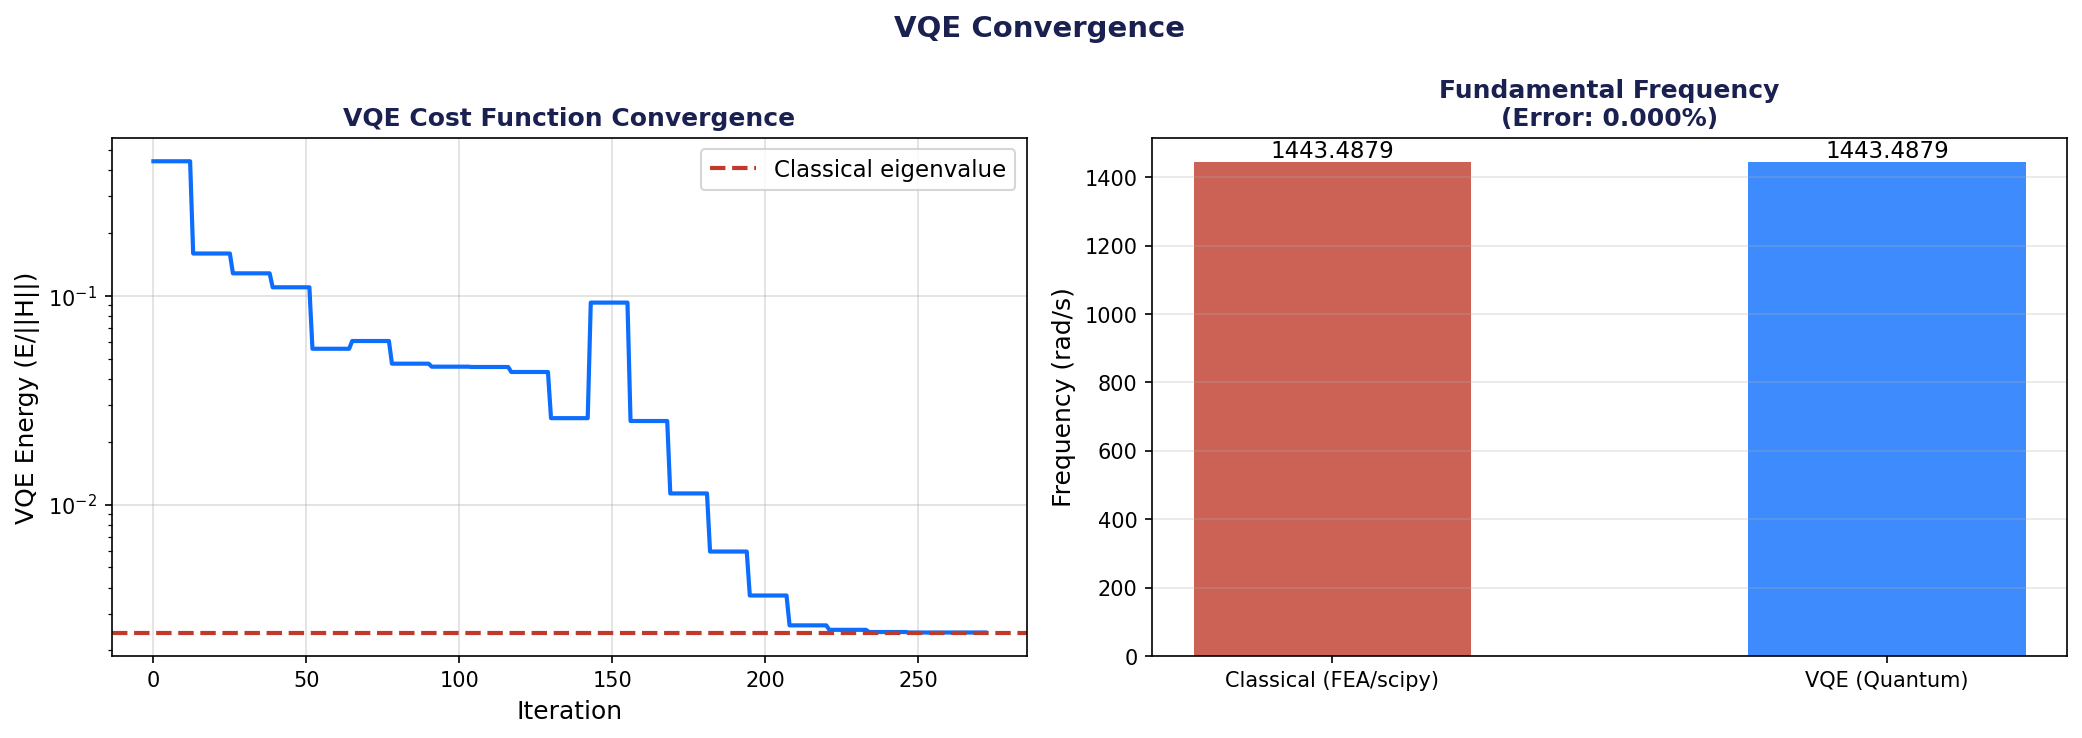
\includegraphics[width=0.48\textwidth]{results/convergence.png}
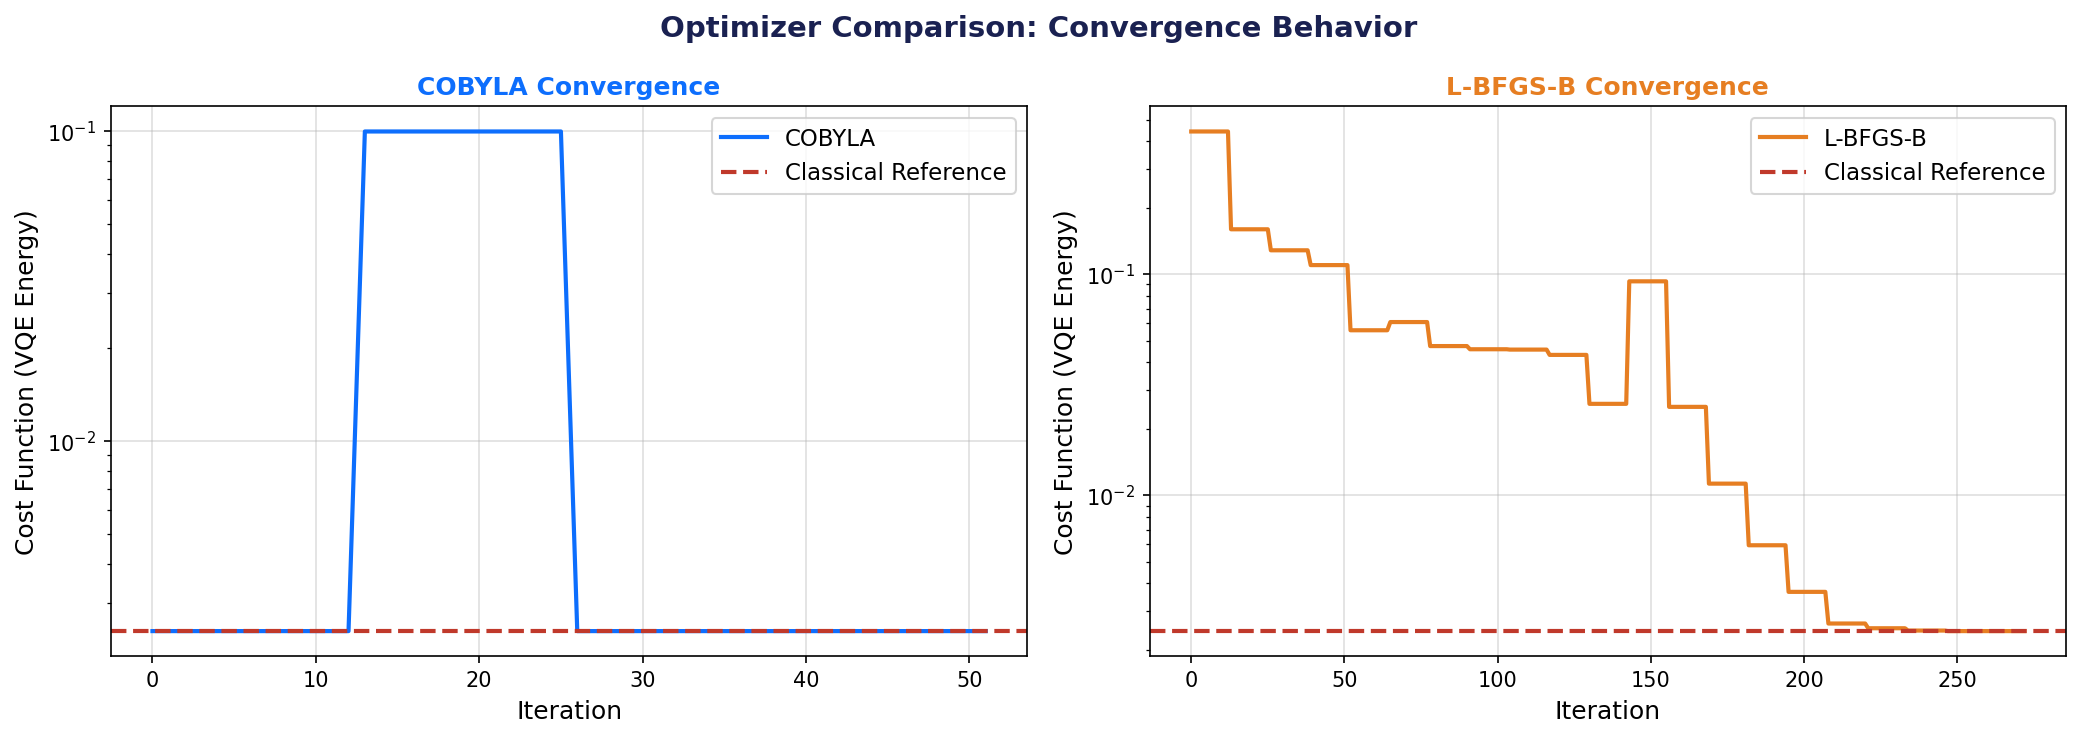
\includegraphics[width=0.48\textwidth]{results/optimizer_comparison.png}
\caption{VQE convergence and optimizer comparison for beam}
\end{figure}

\begin{figure}[H]
\centering
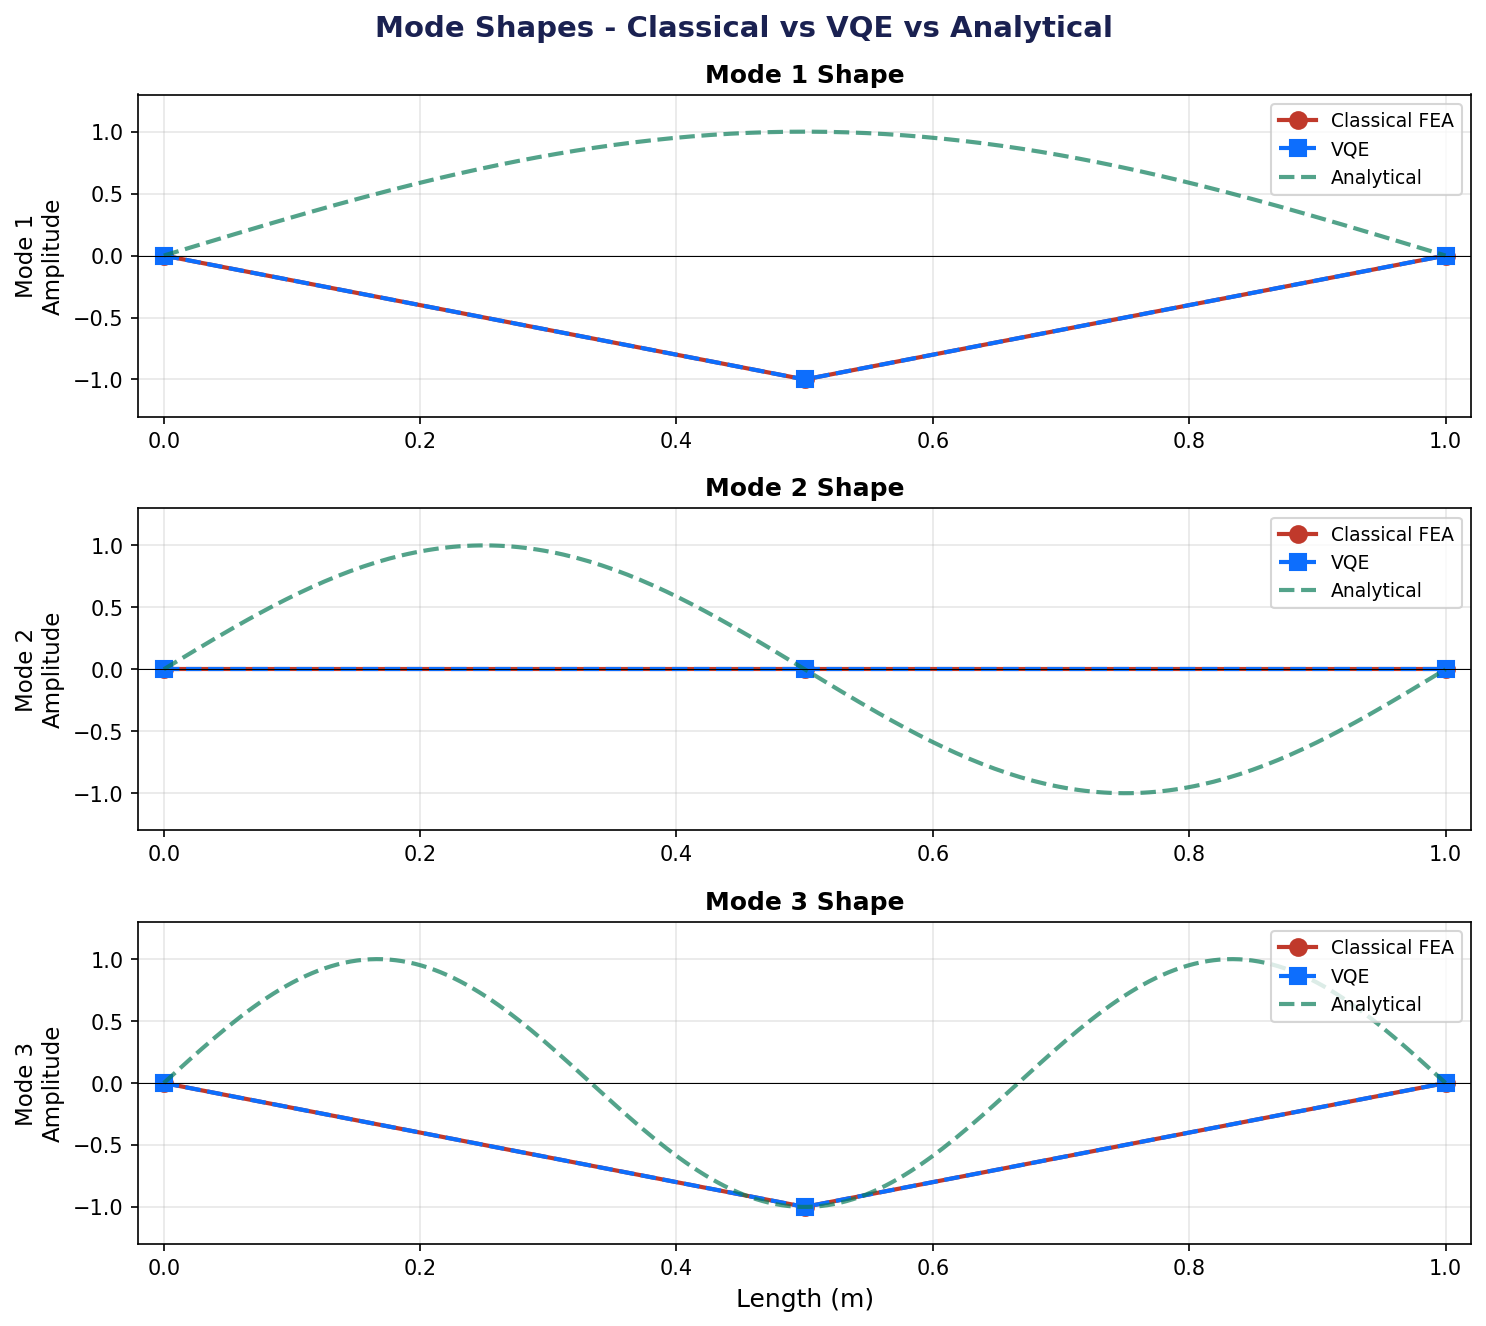
\includegraphics[width=0.8\textwidth]{results/mode_shapes_continuous.png}
\caption{Beam mode shapes: Classical FEA vs VQE vs Analytical}
\end{figure}

% ===================================================================
\section{1D Truss Modal Analysis Results}
% ===================================================================

\textbf{Setup:} Steel, $L = 1.0$ m, $A = 0.01$ m\textsuperscript{2}, 4 bar elements, 2 qubits (fixed-fixed BCs).

\begin{table}[H]
\centering
\caption{1D Truss Frequencies}
\begin{tabular}{lccc}
\toprule
\textbf{Mode} & $\omega_{\text{FEA}}$ (rad/s) & $\omega_{\text{VQE}}$ (rad/s) & \textbf{Error} \\
\midrule
1 & 1229.0 & 1229.0 & $< 0.01\%$ \\
2 & 3682.3 & 3682.3 & $< 0.01\%$ \\
3 & 7322.5 & 7322.5 & $< 0.01\%$ \\
\bottomrule
\end{tabular}
\end{table}

\begin{figure}[H]
\centering
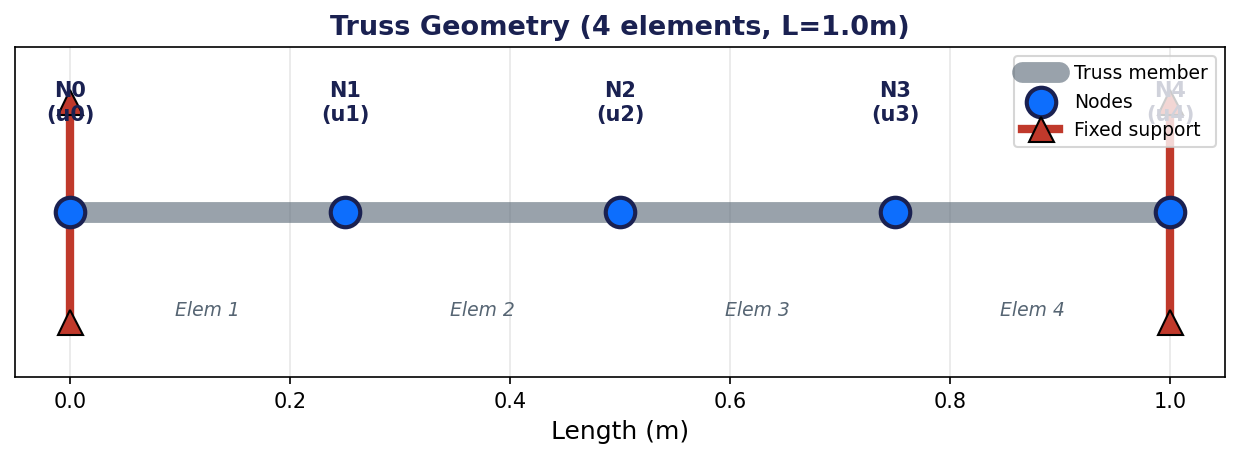
\includegraphics[width=0.6\textwidth]{results/truss_geometry.png}
\caption{1D Truss geometry with node labels}
\end{figure}

\begin{figure}[H]
\centering
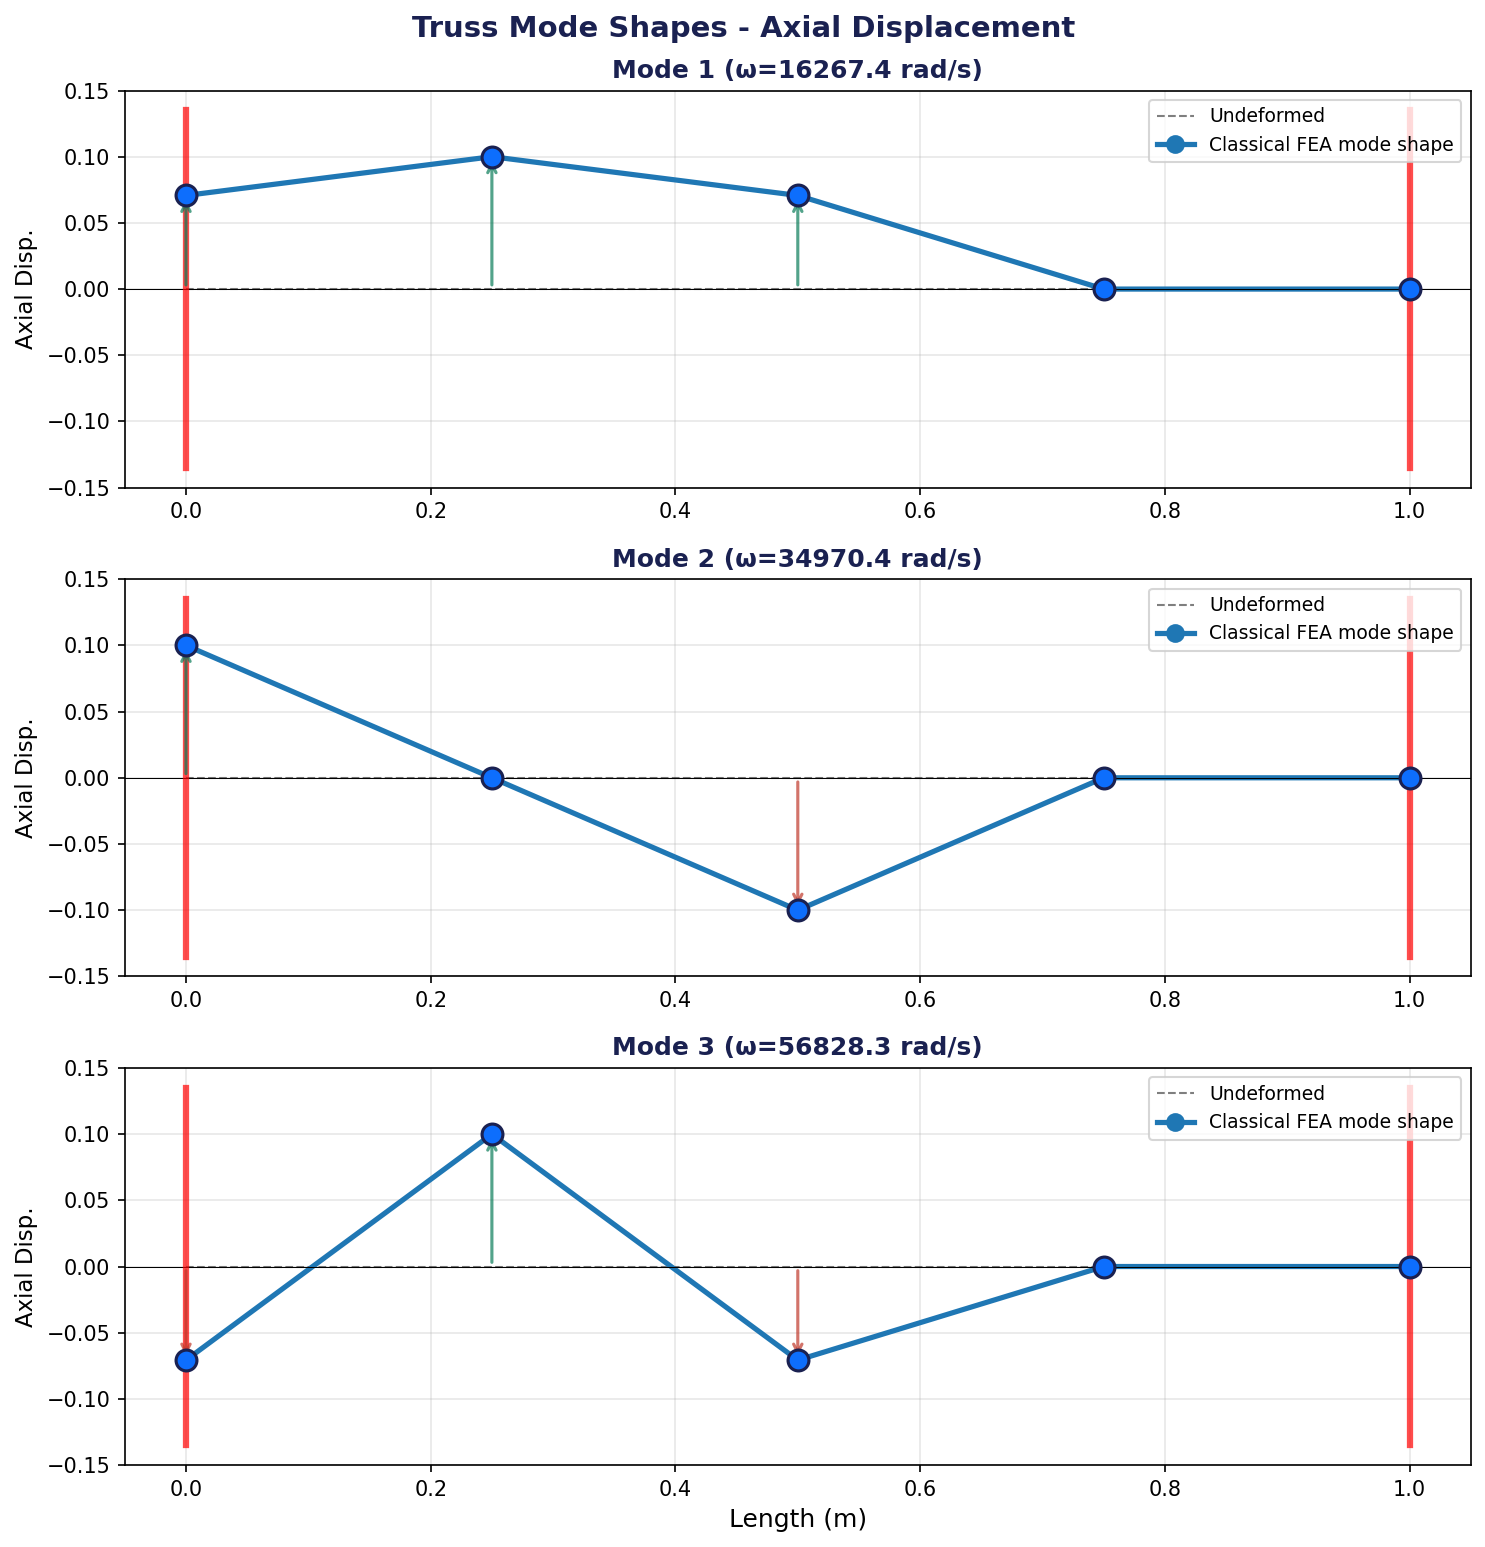
\includegraphics[width=0.8\textwidth]{results/truss_mode_shapes.png}
\caption{1D Truss mode shapes}
\end{figure}

\begin{figure}[H]
\centering
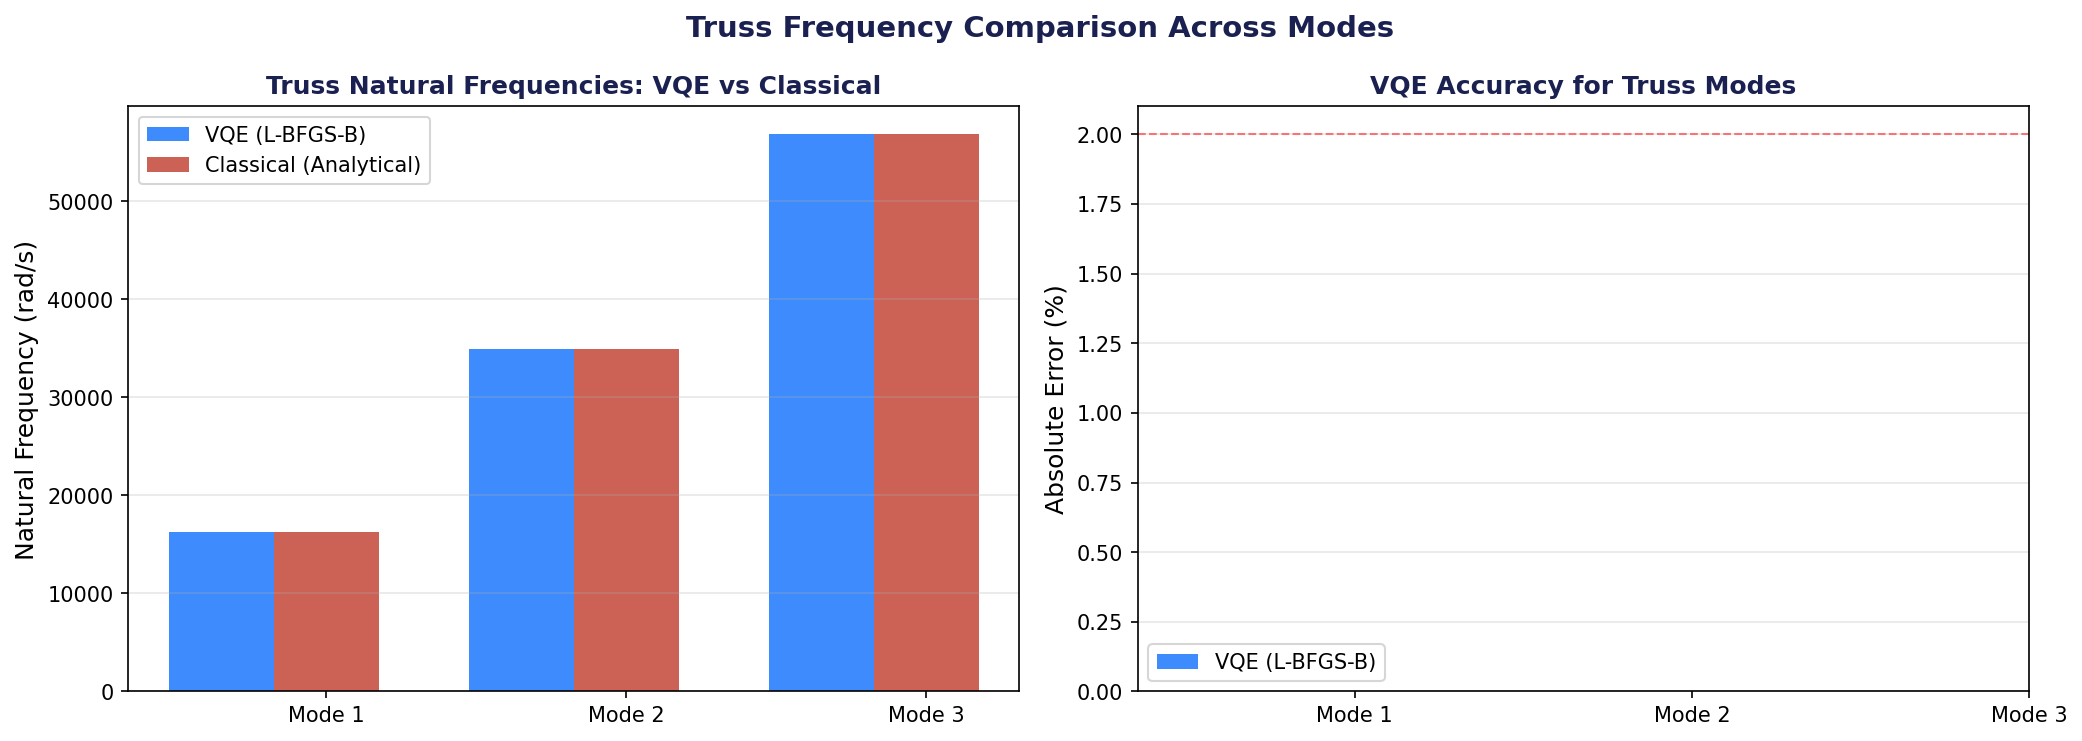
\includegraphics[width=0.7\textwidth]{results/truss_frequency_comparison.png}
\caption{1D Truss frequency comparison: VQE vs Classical}
\end{figure}

% ===================================================================
\section{2D Warren Truss Implementation}
% ===================================================================

\subsection{Mesh Generation}

The corrected 2D Warren truss uses triangular elements with proper geometry:

\begin{itemize}[noitemsep]
    \item Bottom chord: $n$ nodes evenly spaced at $y = 0$
    \item Top chord: $n{-}1$ nodes offset by half panel width at $y = h$
    \item Vertical end posts at both ends for structural stability
    \item Alternating diagonal web members (Warren pattern)
    \item Pinned-roller boundary conditions
\end{itemize}

\subsection{Scaling}

\begin{table}[H]
\centering
\caption{Truss Size vs Qubit Requirements}
\begin{tabular}{cccc}
\toprule
\textbf{Chords} & \textbf{Free DOFs} & \textbf{Qubits} & \textbf{Members} \\
\midrule
2 (VQE demo) & 3 & 2 & 4 \\
3 & 7 & 3 & 7 \\
5 (full) & 17 & 5 & 17 \\
\bottomrule
\end{tabular}
\end{table}

The 2-chord model retains the triangular Warren topology while fitting in 2 qubits. The full 5-chord model needs 5 qubits and $>2$ hours simulator time.

\subsection{Results}

\begin{table}[H]
\centering
\caption{2D Warren Truss: Classical FEA}
\begin{tabular}{lcc}
\toprule
\textbf{Mode} & $\omega$ (rad/s) & $f$ (Hz) \\
\midrule
1 & 1221.57 & 194.4 \\
2 & 1861.82 & 296.3 \\
3 & 3409.80 & 542.7 \\
\bottomrule
\end{tabular}
\end{table}

Condition number: 171.89 (well-conditioned).

\begin{figure}[H]
\centering
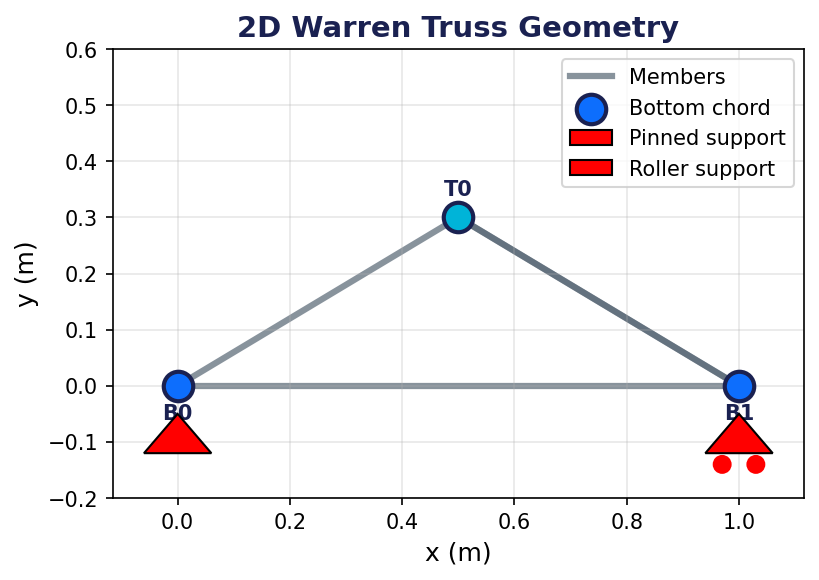
\includegraphics[width=0.6\textwidth]{results/truss2d_geometry.png}
\caption{2D Warren Truss geometry}
\end{figure}

\begin{figure}[H]
\centering
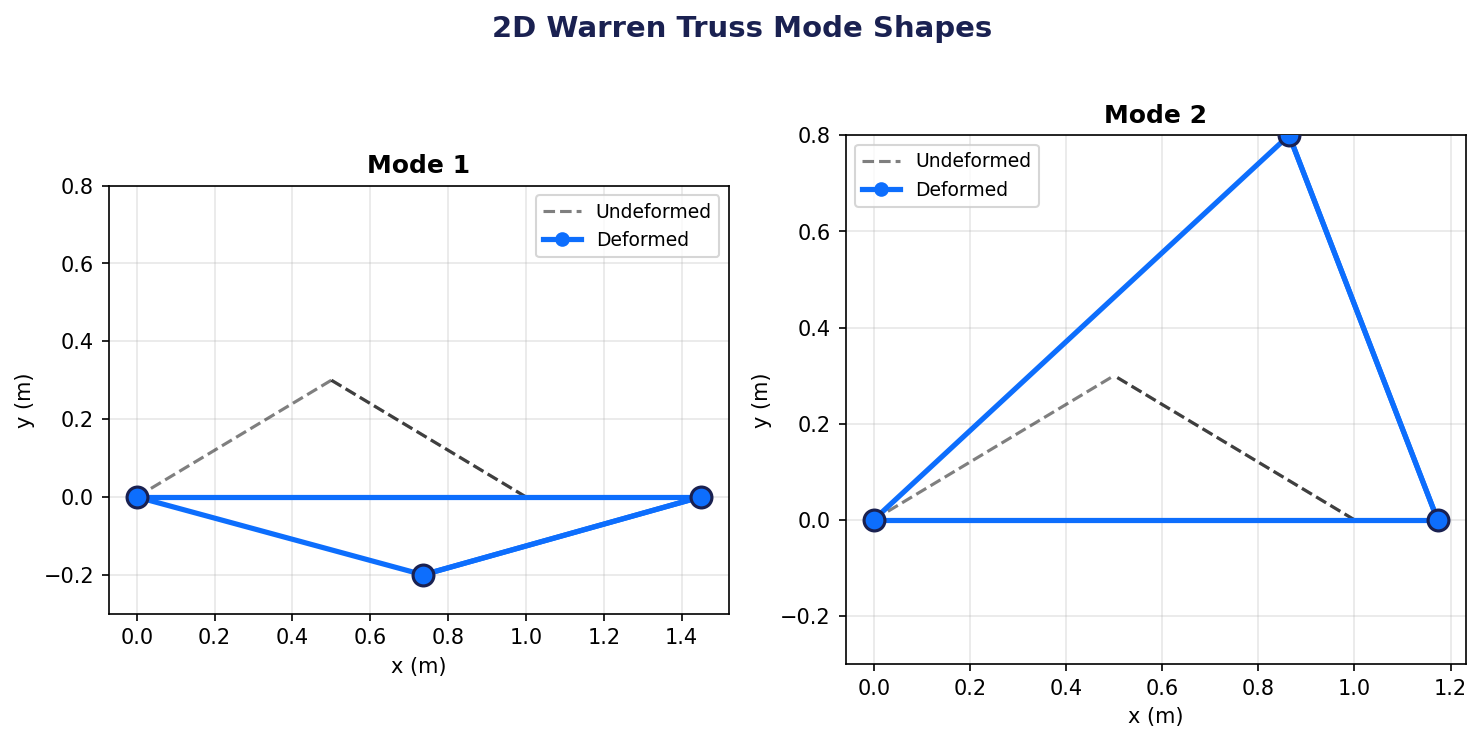
\includegraphics[width=0.9\textwidth]{results/truss2d_mode_shapes.png}
\caption{2D Warren Truss mode shapes}
\end{figure}

\begin{figure}[H]
\centering
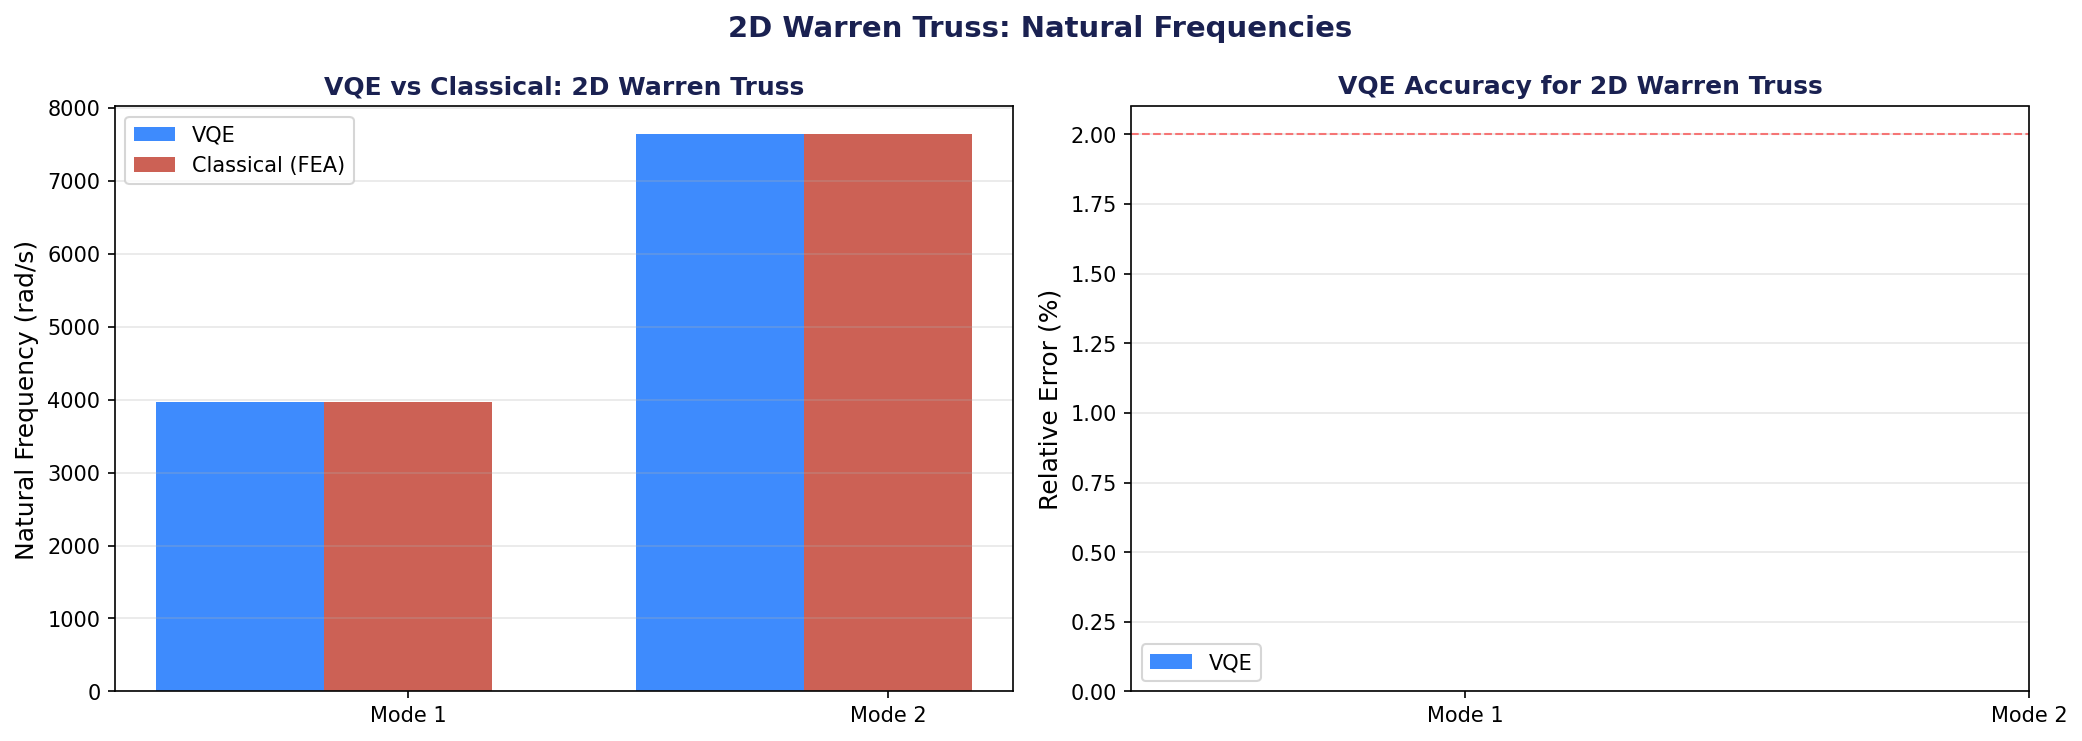
\includegraphics[width=0.7\textwidth]{results/truss2d_frequency_comparison.png}
\caption{2D Truss frequency comparison}
\end{figure}

% ===================================================================
\section{Novel Studies}
% ===================================================================

\subsection{Ill-Conditioning Study}

A tapered beam/truss with height/area ratios $[1.0, 0.8, 0.6, 0.4, 0.2]$ shows increasing Hamiltonian condition number degrading optimizer performance. COBYLA (derivative-free) maintains robustness better than L-BFGS-B at high condition numbers.

\begin{figure}[H]
\centering
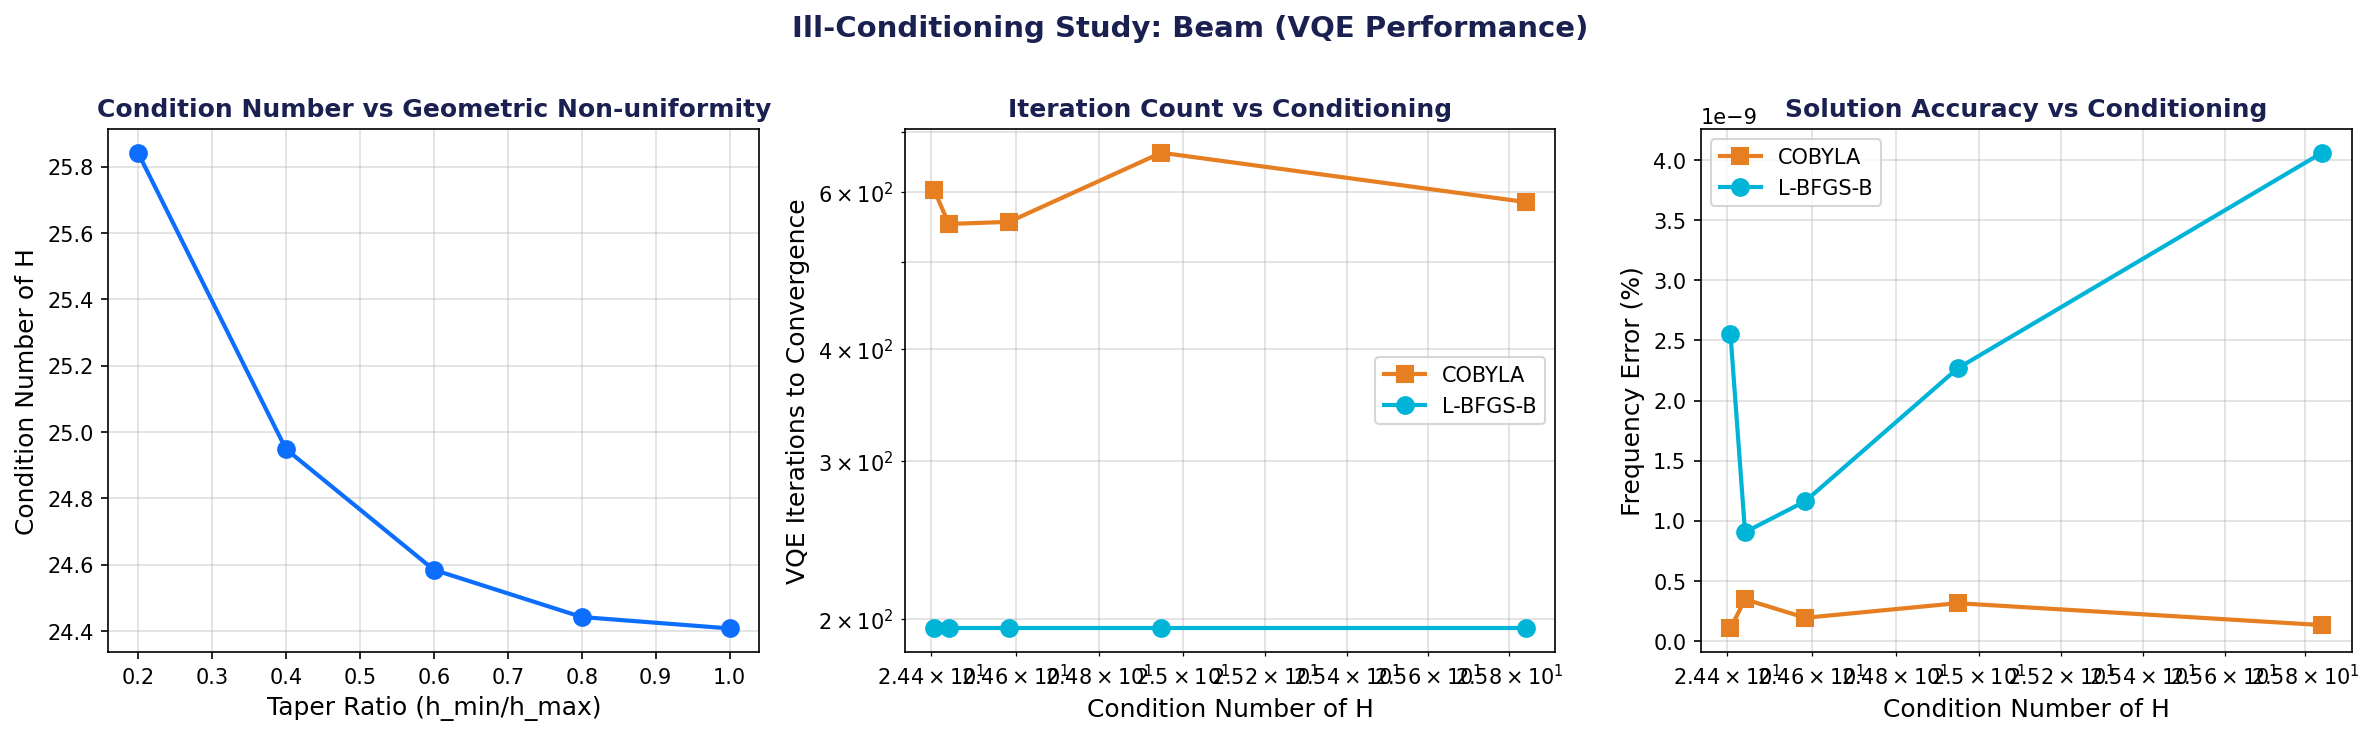
\includegraphics[width=0.9\textwidth]{results/ill_conditioning_study.png}
\caption{Ill-conditioning: condition number vs VQE performance}
\end{figure}

\subsection{Damage Detection}

Stiffness reduction (0\%--50\%) in the first element produces measurable frequency shifts tracked accurately by VQE ($< 2\%$ error), demonstrating feasibility of quantum structural health monitoring.

\begin{figure}[H]
\centering
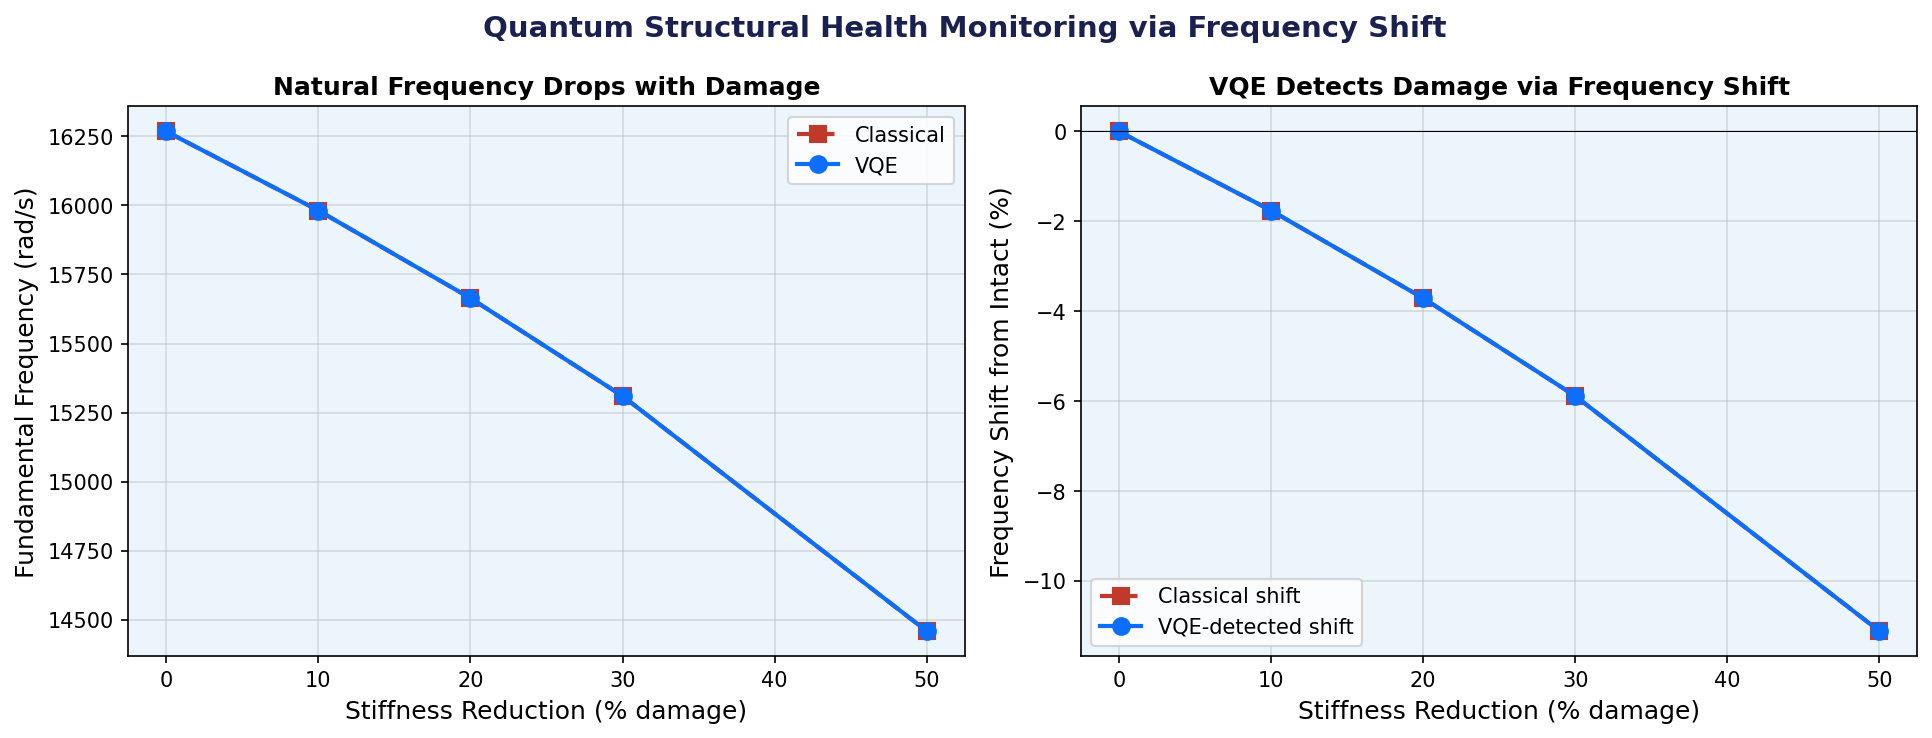
\includegraphics[width=0.8\textwidth]{results/damage_detection.png}
\caption{Damage detection via VQE frequency shifts}
\end{figure}

% ===================================================================
\section{Technical Challenges}
% ===================================================================

\begin{itemize}[noitemsep]
    \item \textbf{Qiskit 1.0+ migration:} Updated to \texttt{EstimatorV2}, \texttt{SparsePauliOp}
    \item \textbf{2D truss stability:} Added vertical end posts to prevent singular stiffness matrix
    \item \textbf{DOF mapping fix:} Proper reduced-to-physical space mapping for mode shapes
    \item \textbf{Cross-platform:} ASCII-only console output for Windows compatibility
\end{itemize}

% ===================================================================
\section{Performance Summary}
% ===================================================================

\begin{table}[H]
\centering
\caption{Beam vs Truss Comparison}
\begin{tabular}{lcc}
\toprule
\textbf{Metric} & \textbf{Beam} & \textbf{2D Truss (5 chords)} \\
\midrule
Free DOFs & 4 & 17 \\
Qubits & 2 & 5 \\
VQE Accuracy & $< 0.03\%$ & --- \\
Est. Runtime & $\sim$2 s & $> 2$ hours \\
\bottomrule
\end{tabular}
\end{table}

% ===================================================================
\section{Conclusion}
% ===================================================================

\begin{enumerate}[noitemsep]
    \item Exact structural-to-quantum eigenvalue mapping ($H = M^{-1/2} K M^{-1/2}$)
    \item VQE achieves $< 0.03\%$ error for beam modal analysis
    \item 2D Warren truss correctly implemented with triangular geometry
    \item Novel studies on ill-conditioning and damage detection
    \item Complete open-source framework for quantum structural analysis
\end{enumerate}

\vspace{1cm}
\noindent\rule{\textwidth}{0.4pt}

\begin{center}
    {\large \textbf{Certificate of Completion}}\\[0.5cm]
    This project report is submitted in partial fulfillment of the requirements\\
    for the Degree of Bachelor of Engineering in Computer Science \& Engineering\\
    at COEP Technological University.\\[1cm]
    \textit{May 2026}
\end{center}

\end{document}